\documentclass{article}

\usepackage{graphicx}
\usepackage{tikz}
\usepackage{tikzsymbols}
\usetikzlibrary{calc,patterns,shapes.geometric}
\pagestyle{empty}
\usepackage[margin=0pt]{geometry}
\geometry{papersize={14in,12in}}

\def\centerarc[#1](#2)(#3:#4:#5){\draw[#1] ($(#2)+({#5*cos(#3)},{#5*sin(#3)})$) arc (#3:#4:#5);}

\begin{document}
	\begin{figure}
		\centering
		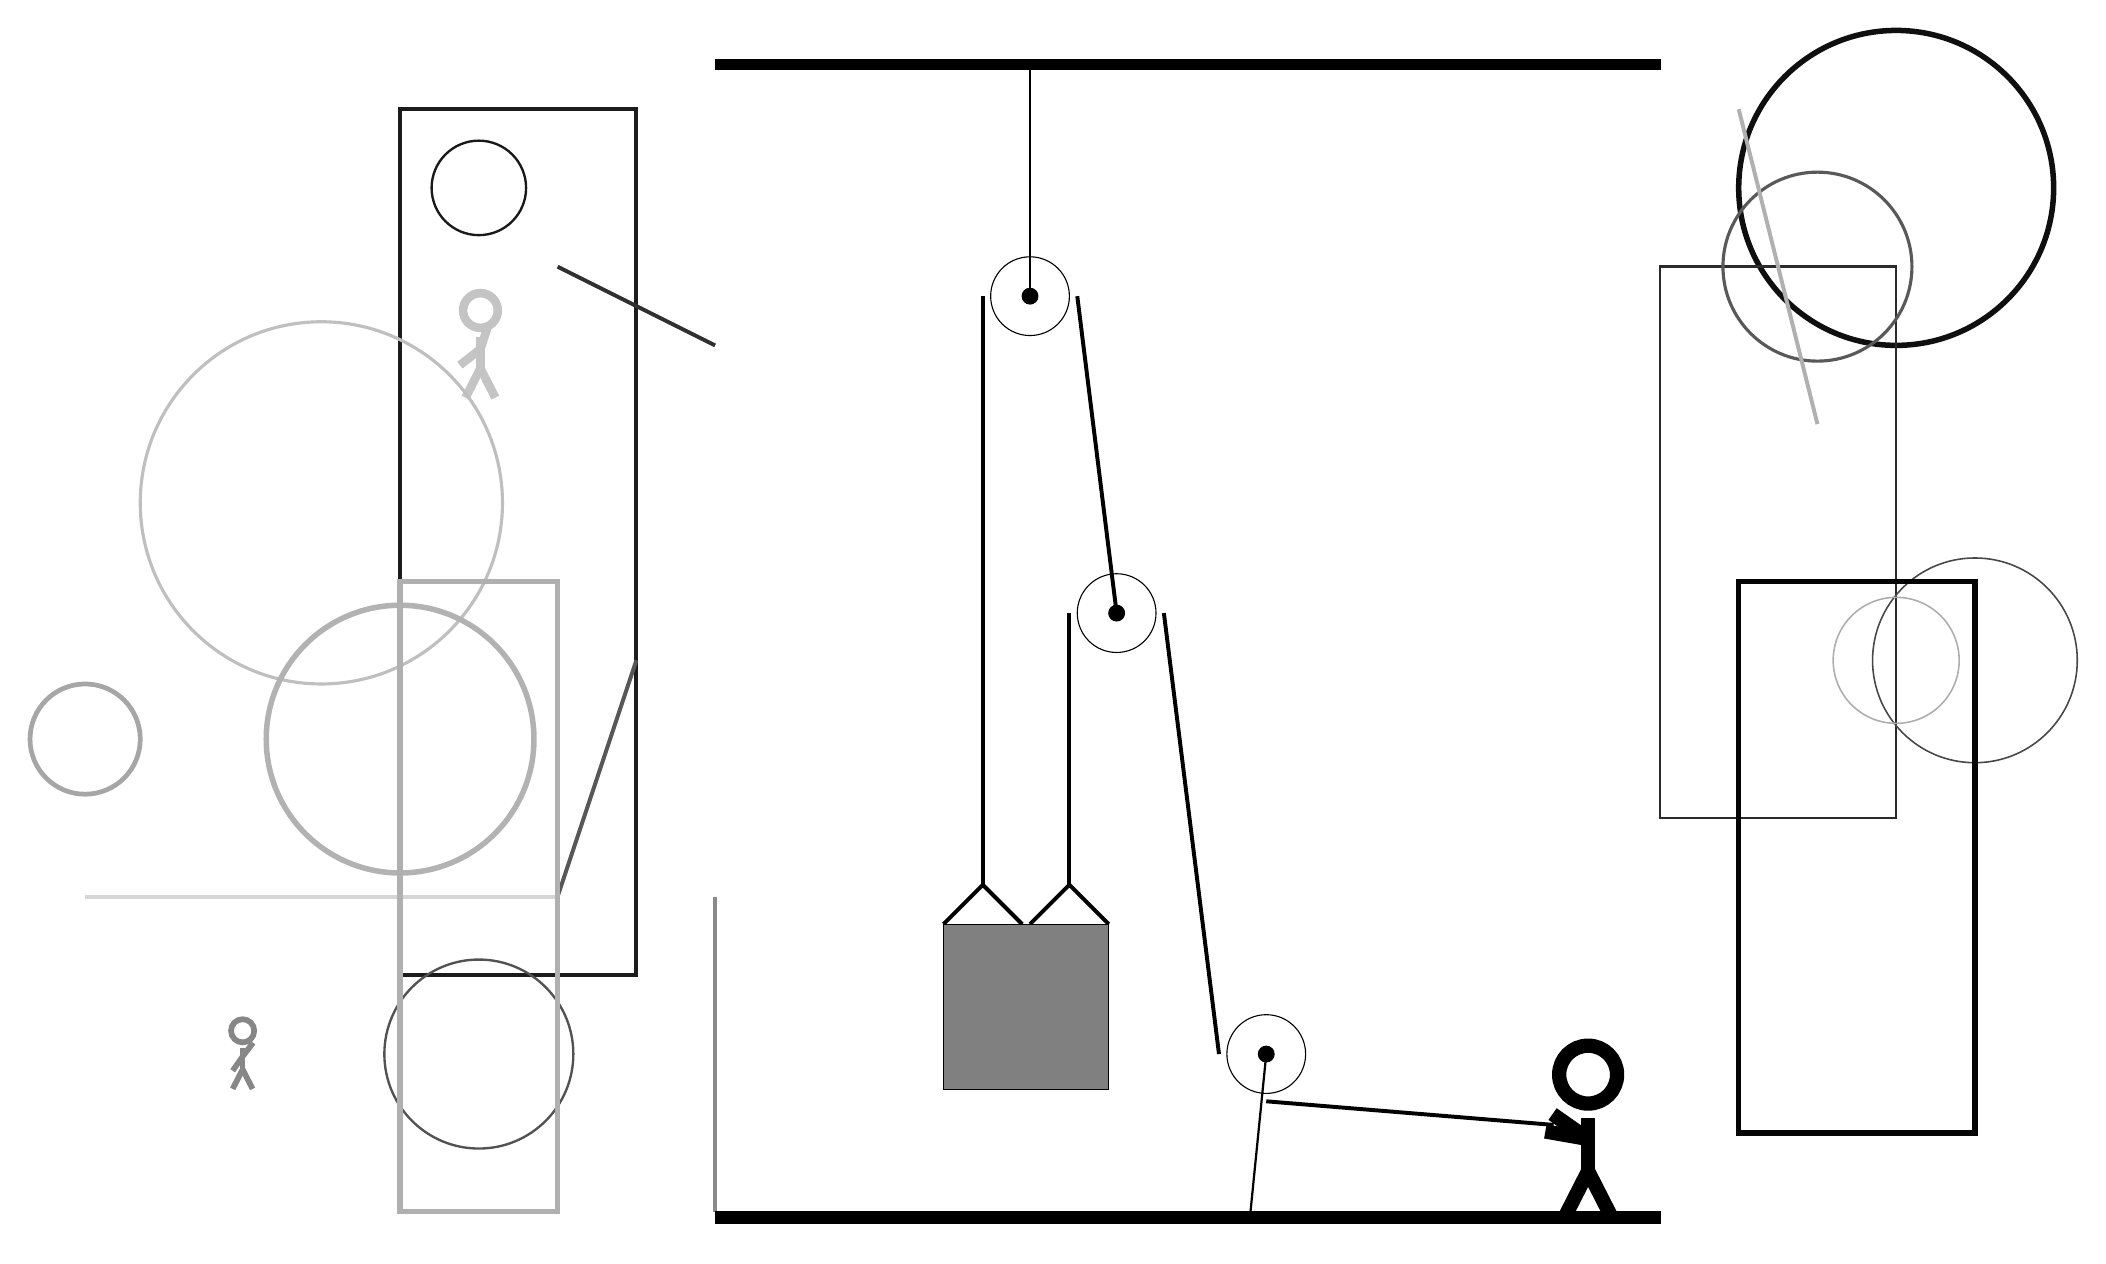
\begin{tikzpicture}
			%%%%% START %%%%%
			
			\draw[fill=black] (-2, 11.5) rectangle (10, 11.625);
			
			\draw (2, 8.625) circle (0.5);
			\draw[fill=black] (2, 8.625) circle (0.1);
			\draw[thick] (2, 8.625) -- (2, 11.5);
			
			\draw[line width=0.5mm, color=black!89] (-3, 11) rectangle (-6, 0);
			
			\draw [line width=0.7mm, color=black!94](13, 10) circle (2.0);
			\draw[line width=0.3mm, color=black!83] (10, 9) rectangle (13, 2);
			\draw[line width=0.5mm, color=black!81](-4, 9) -- (-2, 8);
			
			\draw [line width=0.4mm, color=black!65](12, 9) circle (1.2);
			\draw[line width=0.5mm, color=black!66](-4, 1) -- (-3, 4);
			
			\draw [line width=0.3mm, color=black!90](-5, 10) circle (0.6);
			\draw[line width=0.5mm, color=black!31](12, 7) -- (11, 11);
			\draw[line width=0.5mm, color=black!16](-4, 1) -- (-10, 1);
			\node[line width=0.6mm, color=black!23] at (-5, 8) {\Strichmaxerl[6][38][72]};
			\draw[line width=0.5mm, color=black!46](-2, 1) -- (-2, -3);
			
			\draw [line width=0.4mm, color=black!25](-7, 6) circle (2.3);
			\draw [line width=0.2mm, color=black!72](14, 4) circle (1.3);
			\draw [line width=0.3mm, color=black!68](-5, -1) circle (1.2);
			\node[line width=0.6mm, color=black!47] at (-8, -1) {\Strichmaxerl[4][55][53]};
			\draw [line width=0.7mm, color=black!30](-6, 3) circle (1.7);
			
			\draw [line width=0.6mm, color=black!35](-10, 3) circle (0.7);
			\draw [line width=0.2mm, color=black!32](13, 4) circle (0.8);
			\draw[line width=0.7mm, color=black!98] (11, 5) rectangle (14, -2);
			\draw[line width=0.7mm, color=black!31] (-4, -3) rectangle (-6, 5);
			
			\draw (3.1, 4.6) circle (0.5);
			\draw[fill=black] (3.1, 4.6) circle (0.1);
			
			\draw (5, -1) circle (0.5);
			\draw[fill=black] (5, -1) circle (0.1);
			\draw[thick] (5, -1) -- (4.8, -3);
			
			\draw[line width = 0.5mm]  (0.9, 0.65) -- (1.4, 1.15) -- (1.9, 0.65);
			\draw[line width = 0.5mm]  (2.0, 0.65) -- (2.5, 1.15) -- (3.0, 0.65);
			\draw[fill=black!50] (0.9, 0.65) rectangle (3.0, -1.45);
			
			\draw[line width = 0.5mm] (1.4, 8.625) -- (1.4, 1.15);
			\centerarc[line width = 0.5mm](2, 8.625)(0:180:0.6);
			\draw[line width = 0.5mm] (2.6, 8.625) -- (3.1, 4.6);
			\draw[line width = 0.5mm] (2.5, 4.6) -- (2.5, 1.15);
			\centerarc[line width = 0.5mm](3.1, 4.6)(0:180:0.6);
			\draw[line width = 0.5mm] (3.7, 4.6) -- (4.4, -1);
			\centerarc[line width = 0.5mm](5, -1)(180:270:0.6);
			\draw[line width = 0.5mm] (5, -1.6) -- (8.65, -1.9);
			
			\node at (9, -2) {\Strichmaxerl[10][-35][170]};
			
			\draw[fill=black] (-2, -3) rectangle (10, -3.15);
			
			%%%%% END %%%%%
		\end{tikzpicture}
	\end{figure}	
\end{document}